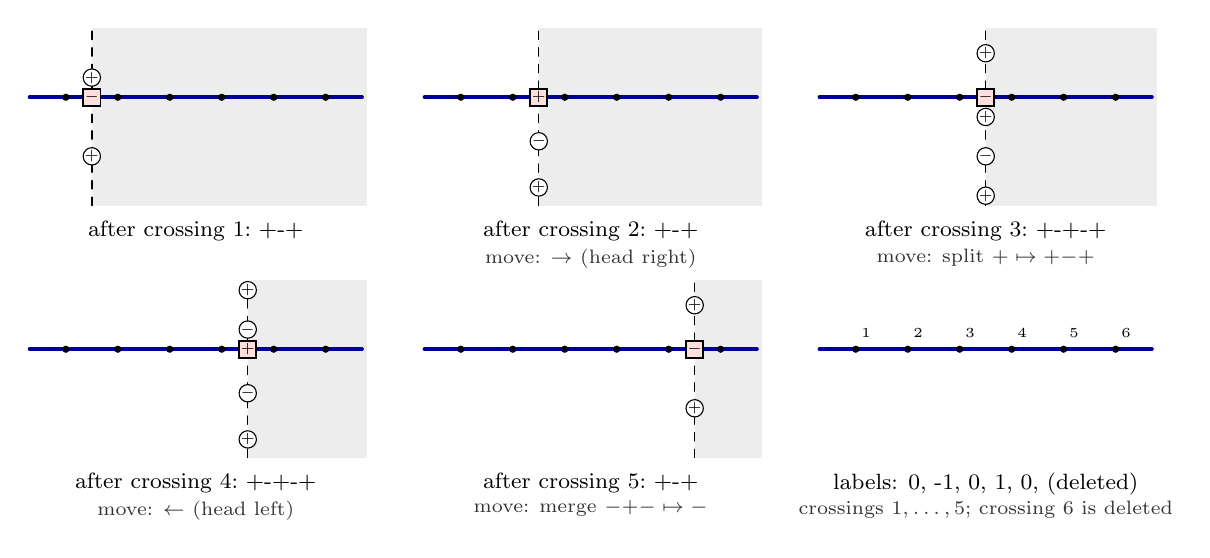
\begin{tikzpicture}[x=0.66cm,y=0.5cm,line cap=round]
\begin{scope}[shift={(0.00,0.00)}]
  \fill[black!7] (1.50,-2.75) rectangle (6.8,1.75);
  \draw[blue!60!black,line width=1.3pt] (0.3,0)--(6.7,0);
  \begin{scope}[black!25,line width=0.6pt]\meanderroad\end{scope}
  \begin{scope}\clip (0.3,-2.75) rectangle (1.50,1.75);\begin{scope}[line width=1pt]\meanderroad\end{scope}\end{scope}
  \draw[dashed,line width=0.5pt] (1.50,-2.75)--(1.50,1.75);
  \foreach \k in {1,...,6} {\fill (\k,0) circle[radius=1.3pt];}
  \draw[fill=white,line width=0.4pt] (1.50,-1.500) circle[radius=0.11cm]; \node[font=\tiny,inner sep=0pt] at (1.50,-1.500) {$+$};
  \draw[fill=red!13,line width=0.7pt] (1.50,0) ++(-0.11cm,-0.11cm) rectangle ++(0.22cm,0.22cm); \node[font=\tiny,inner sep=0pt] at (1.50,0) {$-$};
  \draw[fill=white,line width=0.4pt] (1.50,0.500) circle[radius=0.11cm]; \node[font=\tiny,inner sep=0pt] at (1.50,0.500) {$+$};
  \node[font=\footnotesize,anchor=north] at (3.5,-2.9) {after crossing 1:\ \tape{+}\hd{-}\tape{+}};
\end{scope}
\begin{scope}[shift={(7.60,0.00)}]
  \fill[black!7] (2.50,-2.75) rectangle (6.8,1.75);
  \draw[blue!60!black,line width=1.3pt] (0.3,0)--(6.7,0);
  \begin{scope}[black!25,line width=0.6pt]\meanderroad\end{scope}
  \begin{scope}\clip (0.3,-2.75) rectangle (2.50,1.75);\begin{scope}[line width=1pt]\meanderroad\end{scope}\end{scope}
  \draw[dashed,line width=0.5pt] (2.50,-2.75)--(2.50,1.75);
  \foreach \k in {1,...,6} {\fill (\k,0) circle[radius=1.3pt];}
  \draw[fill=white,line width=0.4pt] (2.50,-2.291) circle[radius=0.11cm]; \node[font=\tiny,inner sep=0pt] at (2.50,-2.291) {$+$};
  \draw[fill=white,line width=0.4pt] (2.50,-1.118) circle[radius=0.11cm]; \node[font=\tiny,inner sep=0pt] at (2.50,-1.118) {$-$};
  \draw[fill=red!13,line width=0.7pt] (2.50,0) ++(-0.11cm,-0.11cm) rectangle ++(0.22cm,0.22cm); \node[font=\tiny,inner sep=0pt] at (2.50,0) {$+$};
  \node[font=\footnotesize,anchor=north] at (3.5,-2.9) {after crossing 2:\ \tape{+}\tape{-}\hd{+}};
  \node[font=\scriptsize,anchor=north,gray!40!black] at (3.5,-3.6) {move: $\to$ (head right)};
\end{scope}
\begin{scope}[shift={(15.20,0.00)}]
  \fill[black!7] (3.50,-2.75) rectangle (6.8,1.75);
  \draw[blue!60!black,line width=1.3pt] (0.3,0)--(6.7,0);
  \begin{scope}[black!25,line width=0.6pt]\meanderroad\end{scope}
  \begin{scope}\clip (0.3,-2.75) rectangle (3.50,1.75);\begin{scope}[line width=1pt]\meanderroad\end{scope}\end{scope}
  \draw[dashed,line width=0.5pt] (3.50,-2.75)--(3.50,1.75);
  \foreach \k in {1,...,6} {\fill (\k,0) circle[radius=1.3pt];}
  \draw[fill=white,line width=0.4pt] (3.50,-2.500) circle[radius=0.11cm]; \node[font=\tiny,inner sep=0pt] at (3.50,-2.500) {$+$};
  \draw[fill=white,line width=0.4pt] (3.50,-1.500) circle[radius=0.11cm]; \node[font=\tiny,inner sep=0pt] at (3.50,-1.500) {$-$};
  \draw[fill=white,line width=0.4pt] (3.50,-0.500) circle[radius=0.11cm]; \node[font=\tiny,inner sep=0pt] at (3.50,-0.500) {$+$};
  \draw[fill=red!13,line width=0.7pt] (3.50,0) ++(-0.11cm,-0.11cm) rectangle ++(0.22cm,0.22cm); \node[font=\tiny,inner sep=0pt] at (3.50,0) {$-$};
  \draw[fill=white,line width=0.4pt] (3.50,1.118) circle[radius=0.11cm]; \node[font=\tiny,inner sep=0pt] at (3.50,1.118) {$+$};
  \node[font=\footnotesize,anchor=north] at (3.5,-2.9) {after crossing 3:\ \tape{+}\tape{-}\tape{+}\hd{-}\tape{+}};
  \node[font=\scriptsize,anchor=north,gray!40!black] at (3.5,-3.6) {move: split $\tape{+}\mapsto\tape{+}\hd{-}\tape{+}$};
\end{scope}
\begin{scope}[shift={(0.00,-6.40)}]
  \fill[black!7] (4.50,-2.75) rectangle (6.8,1.75);
  \draw[blue!60!black,line width=1.3pt] (0.3,0)--(6.7,0);
  \begin{scope}[black!25,line width=0.6pt]\meanderroad\end{scope}
  \begin{scope}\clip (0.3,-2.75) rectangle (4.50,1.75);\begin{scope}[line width=1pt]\meanderroad\end{scope}\end{scope}
  \draw[dashed,line width=0.5pt] (4.50,-2.75)--(4.50,1.75);
  \foreach \k in {1,...,6} {\fill (\k,0) circle[radius=1.3pt];}
  \draw[fill=white,line width=0.4pt] (4.50,-2.291) circle[radius=0.11cm]; \node[font=\tiny,inner sep=0pt] at (4.50,-2.291) {$+$};
  \draw[fill=white,line width=0.4pt] (4.50,-1.118) circle[radius=0.11cm]; \node[font=\tiny,inner sep=0pt] at (4.50,-1.118) {$-$};
  \draw[fill=red!13,line width=0.7pt] (4.50,0) ++(-0.11cm,-0.11cm) rectangle ++(0.22cm,0.22cm); \node[font=\tiny,inner sep=0pt] at (4.50,0) {$+$};
  \draw[fill=white,line width=0.4pt] (4.50,0.500) circle[radius=0.11cm]; \node[font=\tiny,inner sep=0pt] at (4.50,0.500) {$-$};
  \draw[fill=white,line width=0.4pt] (4.50,1.500) circle[radius=0.11cm]; \node[font=\tiny,inner sep=0pt] at (4.50,1.500) {$+$};
  \node[font=\footnotesize,anchor=north] at (3.5,-2.9) {after crossing 4:\ \tape{+}\tape{-}\hd{+}\tape{-}\tape{+}};
  \node[font=\scriptsize,anchor=north,gray!40!black] at (3.5,-3.6) {move: $\leftarrow$ (head left)};
\end{scope}
\begin{scope}[shift={(7.60,-6.40)}]
  \fill[black!7] (5.50,-2.75) rectangle (6.8,1.75);
  \draw[blue!60!black,line width=1.3pt] (0.3,0)--(6.7,0);
  \begin{scope}[black!25,line width=0.6pt]\meanderroad\end{scope}
  \begin{scope}\clip (0.3,-2.75) rectangle (5.50,1.75);\begin{scope}[line width=1pt]\meanderroad\end{scope}\end{scope}
  \draw[dashed,line width=0.5pt] (5.50,-2.75)--(5.50,1.75);
  \foreach \k in {1,...,6} {\fill (\k,0) circle[radius=1.3pt];}
  \draw[fill=white,line width=0.4pt] (5.50,-1.500) circle[radius=0.11cm]; \node[font=\tiny,inner sep=0pt] at (5.50,-1.500) {$+$};
  \draw[fill=red!13,line width=0.7pt] (5.50,0) ++(-0.11cm,-0.11cm) rectangle ++(0.22cm,0.22cm); \node[font=\tiny,inner sep=0pt] at (5.50,0) {$-$};
  \draw[fill=white,line width=0.4pt] (5.50,1.118) circle[radius=0.11cm]; \node[font=\tiny,inner sep=0pt] at (5.50,1.118) {$+$};
  \node[font=\footnotesize,anchor=north] at (3.5,-2.9) {after crossing 5:\ \tape{+}\hd{-}\tape{+}};
  \node[font=\scriptsize,anchor=north,gray!40!black] at (3.5,-3.6) {move: merge $\tape{-}\hd{+}\tape{-}\mapsto\hd{-}$};
\end{scope}
\begin{scope}[shift={(15.20,-6.40)}]
  \draw[blue!60!black,line width=1.3pt] (0.3,0)--(6.7,0);
  \begin{scope}[line width=1pt]\meanderroad\end{scope}
  \foreach \k in {1,...,6} {\fill (\k,0) circle[radius=1.3pt]; \node[fill=white,inner sep=0.5pt,font=\tiny] at (\k+0.2,0.4) {\k};}
  \node[font=\footnotesize,anchor=north] at (3.5,-2.9) {labels: 0,\ -1,\ 0,\ 1,\ 0,\ (deleted)};
  \node[font=\scriptsize,anchor=north,gray!40!black] at (3.5,-3.6) {crossings $1,\dots,5$; crossing $6$ is deleted};
\end{scope}
\end{tikzpicture}
